\documentclass[11pt,oneside]{article}
\usepackage{fullpage}

%%% Load some useful packages:
\usepackage{graphicx}
\graphicspath{{figures/}}
\usepackage{subfigure}
\usepackage{bbm}
\usepackage{tabularx}
\usepackage{setspace}
\onehalfspacing
%% Package to linebreak URLs in a sane manner.
\usepackage{url}

\usepackage{todonotes}
\usepackage{amsmath,amsfonts}
\numberwithin{equation}{subsection}
%% Define a new 'smallurl' style for the package that will use a smaller font.
\makeatletter
\def\url@smallurlstyle{%
  \@ifundefined{selectfont}{\def\UrlFont{\sf}}{\def\UrlFont{\small\ttfamily}}}
\makeatother
%% Now actually use the newly defined style.
\urlstyle{smallurl}

%% Define 'tinyurl' style for even smaller URLs (such as in tables)
\makeatletter
\def\url@tinyurlstyle{%
  \@ifundefined{selectfont}{\def\UrlFont{\sf}}{\def\UrlFont{\scriptsize\ttfamily}}}
\makeatother

%% Provides additional functionality for tabular environments
\usepackage{array}

%% Puts space after macros, unless followed by punctuation
\usepackage{xspace}

%% Make margins less ridiculous
\usepackage{fullpage}

%% Allows insertion of fixme notes for future work
\usepackage[footnote, nomargin]{fixme}

%% Make URLs clickable
\usepackage[colorlinks, bookmarks=true]{hyperref}

\begin{document}
\title{Contribution chapter abstract for Ph.D. dissertation: \\
       \textsc{Software Trajectory Analysis:} \\
       \textsc{An empirically based method for automated software process discovery} \\
       \author{Pavel Senin \\
               Collaborative Software Development Laboratory \\
               Department of Information and Computer Sciences \\
               University of Hawaii \\[0.3cm]
               \texttt{senin@hawaii.edu} \\[0.3cm]
               CSDL Technical Report 09-13 \\
               \url{http://csdl.ics.hawaii.edu/techreports/09-13/09-13.pdf}
       }
       \date{February 2013}
}
\maketitle

\clearpage


\section{Introduction}
Software engineering is a unique area of engineering field having no cost associated with materials
and fabrication, which dominate cost in all other engineering disciplines. 
However, ironically, software engineering is suffering from the costs and challenges
associated with continuous re-design of the software design (development) processes - the issue
which is rarely seen at all in any other engineering areas. 

In order to efficiently deal with this issue, many universal design processes - known as 
software development methodologies - were proposed up to date. 
For example, the Waterfall Model process proposes a sequential pattern in which developers 
first create a Requirements document, then create a Design, then create an Implementation, 
and finally develop Tests. 
In contrast, the Test Driven Development process proposes an iterative pattern,
in which the developer  must first write a test case, then write the code to implement 
that test case, then refactor  the system for maximum clarity and minimal code duplication.

Nevertheless, despite to decades of the development, these universal methodologies known to fail in
delivering of the final product - the software. One of the reasons for these failures thought to be
the immaturity and a somewhat rigid structure of these universal methodologies, which make them
difficult to accomodate change. These, in turn, thought to be the consequences of the traditional,
top-down approach to software process design which requires the developer or manager to ``invent''
the process in the first place. Whether through noticing of recurrent development patterns, or
through a decomposition of a larger process, invention is a difficult task
\cite{citeulike:5043104}. 
Another problem, is that process inventors, limited in their scope, 
always assume an idealized versions of real processes - thus tend to produce ``paper lions'' - 
process models which are likely to be disruptive and  unacceptable for end users, at least 
in their proposed form \cite{citeulike:9758924}. In addition to these facts, the full study 
cycle from a process proposal, through its evaluation, to its full understanding and,
potentially, acceptance is usually measured by years \cite{citeulike:113403}.

In my research, I attempt to contribute to an alternative - the bottom-up - approach to software
process design. The idea ``at large'', is that through the observation of the performed 
by developers processes it is possible to \textit{automatically discover} recurrent behaviors, which
could be further generalized and associated with building blocks of a larger software development
process model. If such a tool is in place, it would significantly improve (by inferring only
real-life behaviors) and shorten in time the process analysis time, and, in addition,
might shed new light on the development process itself.

This idea of inferring a process model through observing and studying performed processes is
not new and was around for decades \cite{citeulike:328044}. The problem with its further
development is usually associated with a number of ``show-stoppers'': the biggest issue is the
privacy concerns, the next is the overall cost of the observations, and the least, but not
the last, is the validity of such studies - it is difficult to make an unbiased judgment in
controlled environment. 

In my work, I am addressing outlined above issues through leveraging of knowledge
discovery techniques applied to software artifact trails. Thus, working with \textit{offline
public data}, I am avoiding privacy concerns and the cost of the surveillance, while, potentially, 
inferring \textit{true behaviors} from the real data.

\section{Background, Previous work}
With transitioning in my research work from Hackystat-collected fine and well-organized data
streams (telemetry streams) to publicly available repositories and often spurious, noisy and
partial data, I encountered a major problem. It turned out, that the phrase, which I wrote in my
thesis proposal - ``...many temporal knowledge discovery and data mining methods developed in the
last decade can be applied to the software process domain...'' - was a bit of overstatement. During 
the evaluation of methods on the real data, most of them produce insensible results,
especially non-data adaptive ones - those which are based on the sequential events analysis, or
assume a periodicity.

While these would be my own, speculative statement coming from my own experience, the failure of
common sequential or associative pattern mining techniques can be directly contributed to the
inconsistency ant granularity of public data. The numerous software process artifacts, that I
have collected from public software repositories, just do not reflect all those, essential for
mining atomic events such as coding, compiling, building, and testing.
Moreover, events which are possible to recognize, such as change, are misplaced in time
and very often merged together by the commit process. (I have tried a number of techniques:
Apriori-like algorithms, state-machines like technique based on ProM)

The failure of time series analysis techniques based on the periodicity and consistent ordering
happens due to the intrinsic aperiodicity and disordered nature of developers behaviors.
Humans do not work on a \textit{pre-defined periodic schedule} - we have all sorts of distractions 
during development time - phone calls, meetings, co-workers popping in, emails, etc.
Developers could take a sick leave, or just take a day off to go to the football game,
or just get stuck solving a programming problem, or pause a project juggling priorities.
Also, without any time and space constraints placed on the workplace - in the contemporary
``connected'' world - developers do code literally at the middle of the night, or during
long commute on train, or while on an airplane. Here, from my experience, techniques based on
Fourier decomposition performed poorly.

In order to advance in the pointed in my proposal direction, I had no other choice, but turn to
literature again. Fortunately, through experiments with symbolic approximation 

ing with design a
generic process analysis methodology built upon a novel technique for knowledge discovery from
temporal data, evaluated its performance, and conducted an exploratory study of software process
discovery from software artifact trails based on
three use cases. That is these two pieces - the novel technique of knowledge discovery from
temporal data, and the exploratory study of its application to software development artifacts
trails are the main contributions of my thesis.

After all, we must assume here, that the data I am working with in this thesis is not
only large, but incomplete, displaced in time, noisy, spurious and aperiodic. Moreover, it is
important to understand, that this data is essentially a product of two components. First component
is a behavioral one - the human-driven, non-recurrent, aperiodic, creative process of coding, while
second component is the technology and methodology in use. While latter probably provides a
potentially well-measurable, marginal effect, it is still another source of noise in the data since
there a very little is known about each individual settings from software process artifacts.

Apparently, with this assumptions in place, there are very few possibilities
left, consider the Figure \ref{fig:timeseries-representations} showing common time series data
representations suitable for analyses.

\begin{figure}[tbp]
   \centering
   \includegraphics[height=40mm]{representations.eps}
   \caption{A hierarchy of all the various time series representations in the literature from
       \cite{citeulike:2821475}. The leaf nodes refer to the actual representation, and the internal
            nodes refer to the classification of the approach.}
   \label{fig:timeseries-representations}
\end{figure}

Fortunately, by extending a latest symbolic approximation technique - SAX, and by combining it with
a well-known in the information retrieval field TF*IDF statistics and the Vector space model, I was
able to design a very well performing algorithm for temporal patterns discovery which I present in
the Section \ref{JMotif}. This algorithm not only performs on par and superior to current
state of the art, but is capable of producing interpretable results. Yet, another benefit of the
proposed technique is that it facilitates clustering.

\subsection{Mining software process artifacts trails}
Software artifacts are abundant and thought to carry a significant amount of information about
performed processes. However, the vast majority of artifacts are concerned about the software itself
and largely associated  with a specific development methodology. Examples of such artifacts are
design documents, use cases, class diagrams and requirements, user manuals, etc. The payload of this
artifacts aids in understanding of a function, architecture, and the design of software, while
carrying a very little information about the applied effort and underlying behaviors. 

Due to this fact, I put the content of such artifacts outside of my immediate attention,
however, their layout in time - the density of their appearance, change, and death, are under
analysis.

Let me step back a bit here and explain a larger picture: the process recognition is built upon two
fundamental tasks: description and classification. Given a process, a recognition system first
generates a description of it (i.e., reconstructs the process in full or partially) and then
classifies the process based on that description (i.e., the recognition).

There are two general approaches for implementing such recognition systems - statistical and
structural. These employ different techniques for description and classification. Statistical
approaches to process recognition use theoretical concepts to discriminate among objects belonging
to different groups based upon their quantitative features. Structural approaches use syntactic
grammars to discriminate among objects belonging to different groups based upon the arrangement of
their morphological (structural organization) features. Finally, there are hybrid approaches to
pattern recognition combining aspects of both statistical and structural pattern recognition. This
last, hybrid approach I will take in the thesis.

The reasons for taking this route were explained above - the insufficient granularity of
available information and its spurious temporal arrangement. Thus, instead of inferring
process structures by ordering observed events, I rather look on these events densities and, by
using the statistical apparatus, I relate these patterns to performed activities. 

The idea is that 
By using larger
time intervals, 

Then, these

building structural
iasI focus on the layout of activities in time and their density. By using 


Many engineering, scientific, and production fields (such as movie-making or advertisement) have explicit 
and formalized design processes which are well studied to at least some degree. In contrast, in software 
development we are treating the process of design itself as a thing to be designed and, potentially, 
re-designed along the way. While there are ``best practices'', they prone to fail and it is commonplace
to alter these through combination or a systematic change.



Software artifacts are abundant and thought to carry a significant amount of information about performed 
processes.

However, the vast majority of artifacts are concerned about the software itself and largely associated 
with a specific development methodology. Examples of such artifacts are design documents, use cases, class 
diagrams and requirements, user manuals, etc. The payload of this artifacts aids in understanding of 
a function, architecture, and the design of software, while carrying a very little information about the 
applied effort and underlying behaviors. Due to this fact, I put such artifacts outside of this thesis
immediate attention.

What is studied in this work, is the informational content of software development process byproducts 
which accompany software change. It is long known that change Change not only provides an evidence about performed activities, and, potentially, 
carry an informational load about
recurrent behaviors. Such artifacts span in time, as behaviors do, and usually reflect both: the applied 
effort (process), and the evolution of the software itself. 
Examples of such artifacts are source code changes, bug reports, and developers discussions.

Note, however, that developers do not intentionally create these artifacts to enable research, or to keep 
things in some order - mainly, these artifacts are the pure byproduct helping to the development of a 
software project. Thus, we must assume here, that this data is inconsistent, that any kind of annotations 
used by developers might be erroneous, and the amount of disclosed information could simply be not enough
to determine the actual generative behavior - which ultimately leads to uncertainty of any claims about
process correctness, ``productivity'', or any other performance-related metrics. 

The focus of my work is to explore the informational content of software process artifacts designing 
a toolkit capable to handle the discovery of recurrent behaviors automatically. Ideally, such a toolkit 
must have following properties:
\begin{itemize}
 \item it must be Effective: the reported findings, with respect to behaviors reconstruction, must agree 
 with human intuition.
 \item it should be Scalable: currently software process artifact trails for a single project could easily 
       grow beyond dozens of gigabytes, thus, the computation technique should ideally be able to utilize 
       parallelization and be capable to pre-compute intermediate results alleviating the overall space-time 
       complexity to enable an online (fast turn-around) interactive mining.
 \item Efficient: the set of reported findings should not exceed a certain threshold simly becoming an 
        overwhelming stream of spurious facts.
\end{itemize}


\section{Methodology} \label{JMotif}
Given multiple trails of software process artifacts, how to find recurrent behaviors? In this chapter, 
I will describe the design and an implementation of research methodology employed in Software Trajectory 
Analysis. In short, the implemented approach enables aggregation, indexing and mining of software 
artifact trails allowing the discovery of recurrent behaviors. 

\section{Temporal attributes of software process artifacts}
The close examination and analysis of temporal dynamics of artifact-generating events laying the foundation 
of STA methodology. The extraction of software process-related metrics, their temporal partitioning and the
ability of finding the relevant information is the 



%%% Input file for bibliography
\bibliography{seninp}
%% Use this for an alphabetically organized bibliography
\bibliographystyle{plain}
%% Use this for a reference order organized bibliography
%\bibliographystyle{unsrt}
%% Try using this BibTeX style that hopefully will print annotations in
%% the bibliography. This will allow me to make notes on papers in the
%% BibTeX file and have them readable in the references section until
%% I turn them into a conceptual literature review 
%\bibliographystyle{annotation}

\end{document}
